\documentclass[a4paper]{article}
\usepackage{setspace}
\usepackage[T2A]{fontenc} %
\usepackage[utf8]{inputenc} % подключение русского языка
\usepackage[russian]{babel} %
\usepackage[12pt]{extsizes}
\usepackage{mathtools}
\usepackage{graphicx}
\usepackage{fancyhdr}
\usepackage{amssymb}
\usepackage{amsmath, amsfonts, amssymb, amsthm, mathtools}
\usepackage{tikz}

\usetikzlibrary{positioning}
\setstretch{1.3}

\newcommand{\mat}[1]{\begin{pmatrix} #1 \end{pmatrix}}
\newcommand{\vmat}[1]{\begin{vmatrix} #1 \end{vmatrix}}
\renewcommand{\f}[2]{\frac{#1}{#2}}
\newcommand{\dspace}{\space\space}
\newcommand{\s}[2]{\sum\limits_{#1}^{#2}}
\newcommand{\mul}[2]{\prod_{#1}^{#2}}
\newcommand{\sq}[1]{\left[ {#1} \right]}
\newcommand{\gath}[1]{\left[ \begin{array}{@{}l@{}} #1 \end{array} \right.}
\newcommand{\case}[1]{\begin{cases} #1 \end{cases}}
\newcommand{\ts}{\text{\space}}
\newcommand{\lm}[1]{\underset{#1}{\lim}}
\newcommand{\suplm}[1]{\underset{#1}{\overline{\lim}}}
\newcommand{\inflm}[1]{\underset{#1}{\underline{\lim}}}
\newcommand{\Ker}[1]{\operatorname{Ker}}

\renewcommand{\phi}{\varphi}
\newcommand{\lr}{\Leftrightarrow}
\renewcommand{\l}{\left(}
\renewcommand{\r}{\right)}
\newcommand{\rr}{\rightarrow}
\renewcommand{\geq}{\geqslant}
\renewcommand{\leq}{\leqslant}
\newcommand{\RR}{\mathbb{R}}
\newcommand{\CC}{\mathbb{C}}
\newcommand{\QQ}{\mathbb{Q}}
\newcommand{\ZZ}{\mathbb{Z}}
\newcommand{\VV}{\mathbb{V}}
\newcommand{\NN}{\mathbb{N}}
\newcommand{\OO}{\underline{O}}
\newcommand{\oo}{\overline{o}}
\renewcommand{\Ker}{\operatorname{Ker}}
\renewcommand{\Im}{\operatorname{Im}}
\newcommand{\vol}{\text{vol}}
\newcommand{\Vol}{\text{Vol}}

\DeclarePairedDelimiter\abs{\lvert}{\rvert} %
\makeatletter                               % \abs{}
\let\oldabs\abs                             %
\def\abs{\@ifstar{\oldabs}{\oldabs*}}       %

\begin{document}

\section*{Домашнее задание на 10.04 (Линейная алгебра)}
 {\large Емельянов Владимир, ПМИ гр №247}\\\\
\begin{enumerate}
    \item[\textbf{№1}]Найдём ФСР однородной системы линейных уравнений:
    $$\case{
        x_1 - x_2 + x_4 = 0\\
        x_2 + x_3 - x_4 = 0
    }\implies \mat{x_1\\x_2\\x_3\\x_4} = \mat{-x_3\\-x_3+x_4\\x_3\\x_4} = \mat{-1\\-1\\1\\0}x_3 + \mat{0\\1\\0\\1}x_4$$
    Базис $S$:
    $$\left\{\mat{-1\\-1\\1\\0},  \mat{0\\1\\0\\1}\right\}$$
    Точка из $L$:
    $$(2, 0, 1, 0)$$


    \item[\textbf{№2}]$$\case{x = 3-t\\y=-1+4t} \lr 4x + y -11=0 \lr \f{x-3}{-1}=\f{y+1}{4}$$
    Направляющий вектор и нормаль:
    $$\vec{a} = (-1, 4), \quad \vec{n} = (4, 1)$$
    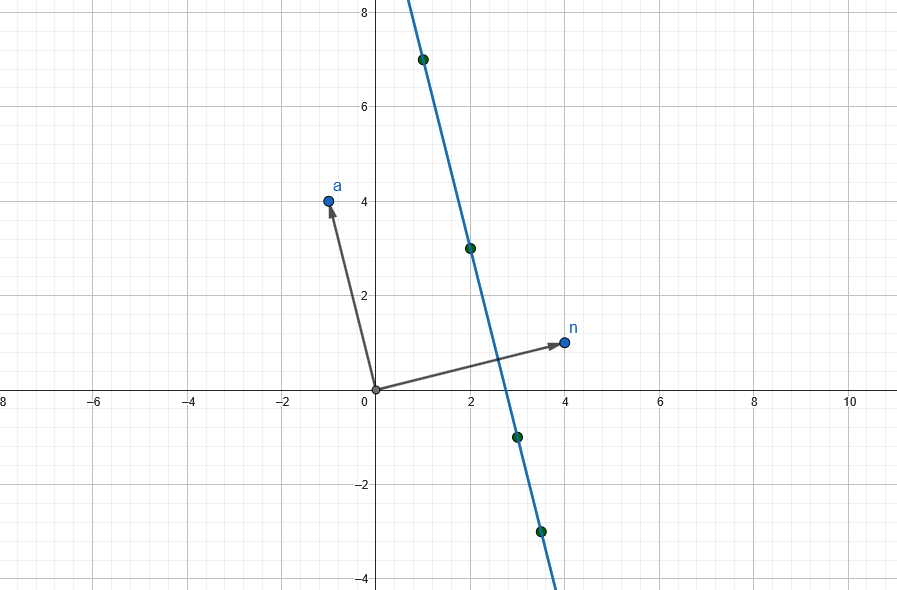
\includegraphics[scale=0.6]{image.png}\\

    \item[\textbf{№3}]Найдём:
    $$\vmat{x-2 & y-3 & z- 1 \\ 3 -2 & 1 - 3 & 4 - 1\\ 2 -2 & 1-3 & 5-1} = 18 - 2x - 4y - 2z = 0$$
    \textbf{Ответ:} $9 - x - 2y - z=0$
\end{enumerate}
\end{document}